\begin{frame}{Numerical Results}{Classical simulation setup}
    % \item Results produced using classical simulation of QAOA in Qiskit
    % \item Simulation limited to $\leq 27$ qubits on local hardware
    % \begin{itemize}
    %     \item $(|V|=10, |E|=22)$
    %     \item $(|V|=20, |E|=42)$
    % \end{itemize}
    % Parameters varied:
    \begin{itemize}
        \item Number of requests: $2$ to $10$
        \item Number of alternate routes: $1$ to $10$
        \item Number of wavelengths: $1$ to $\abs{P}$
        \item Circuit depths $1$ to $4$
        \item Two network topologies
        \item Result compared to the $k$ shortest paths first-fit
    \end{itemize}
    % \item 142 RWA instances, depths $p=1$ to $p=4$
    % \item Baseline: $k$-shortest-path first-fit (k-SPFF)
    % \item Two random network topologies:
\begin{figure}[!htbp]
	\centering
	\begin{subfigure}{0.4\textwidth}
	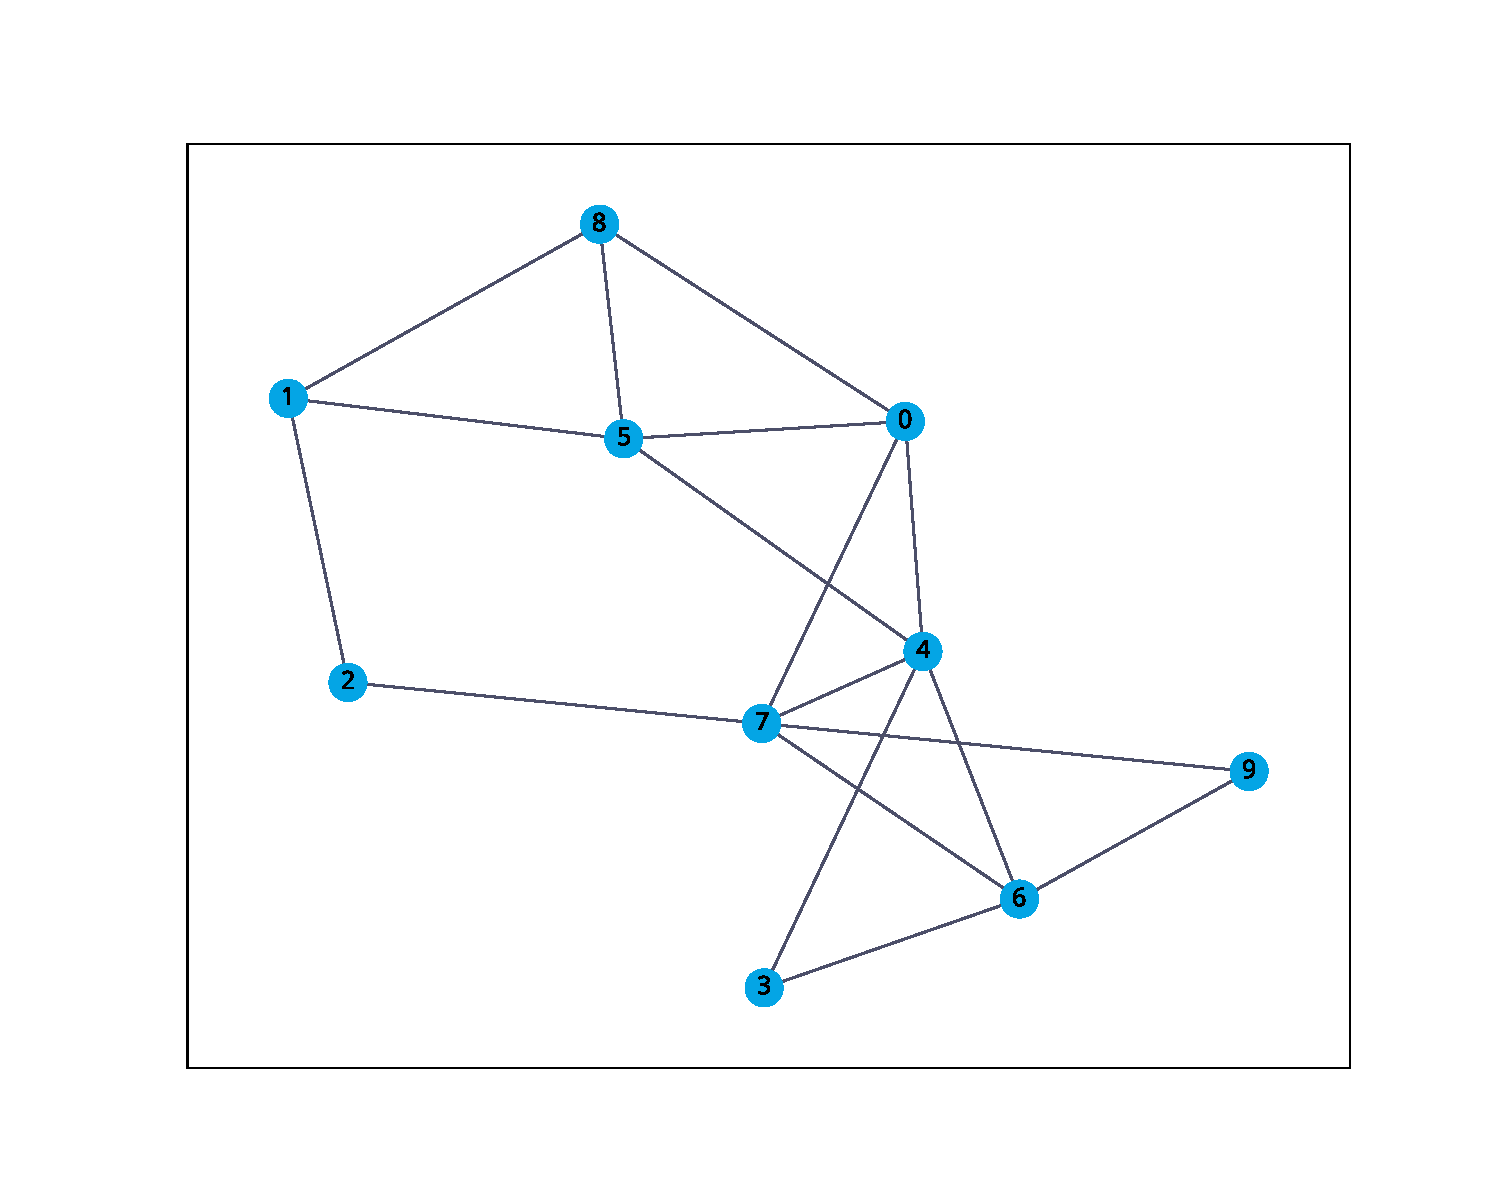
\includegraphics[width=\textwidth]{pictures/plots/10.pdf}
	\caption{\scriptsize$\abs{V} = 10$ nodes and $\abs{E} = 22$ links. (Small)}
	\end{subfigure}
	\quad
	\begin{subfigure}{0.4\textwidth}
	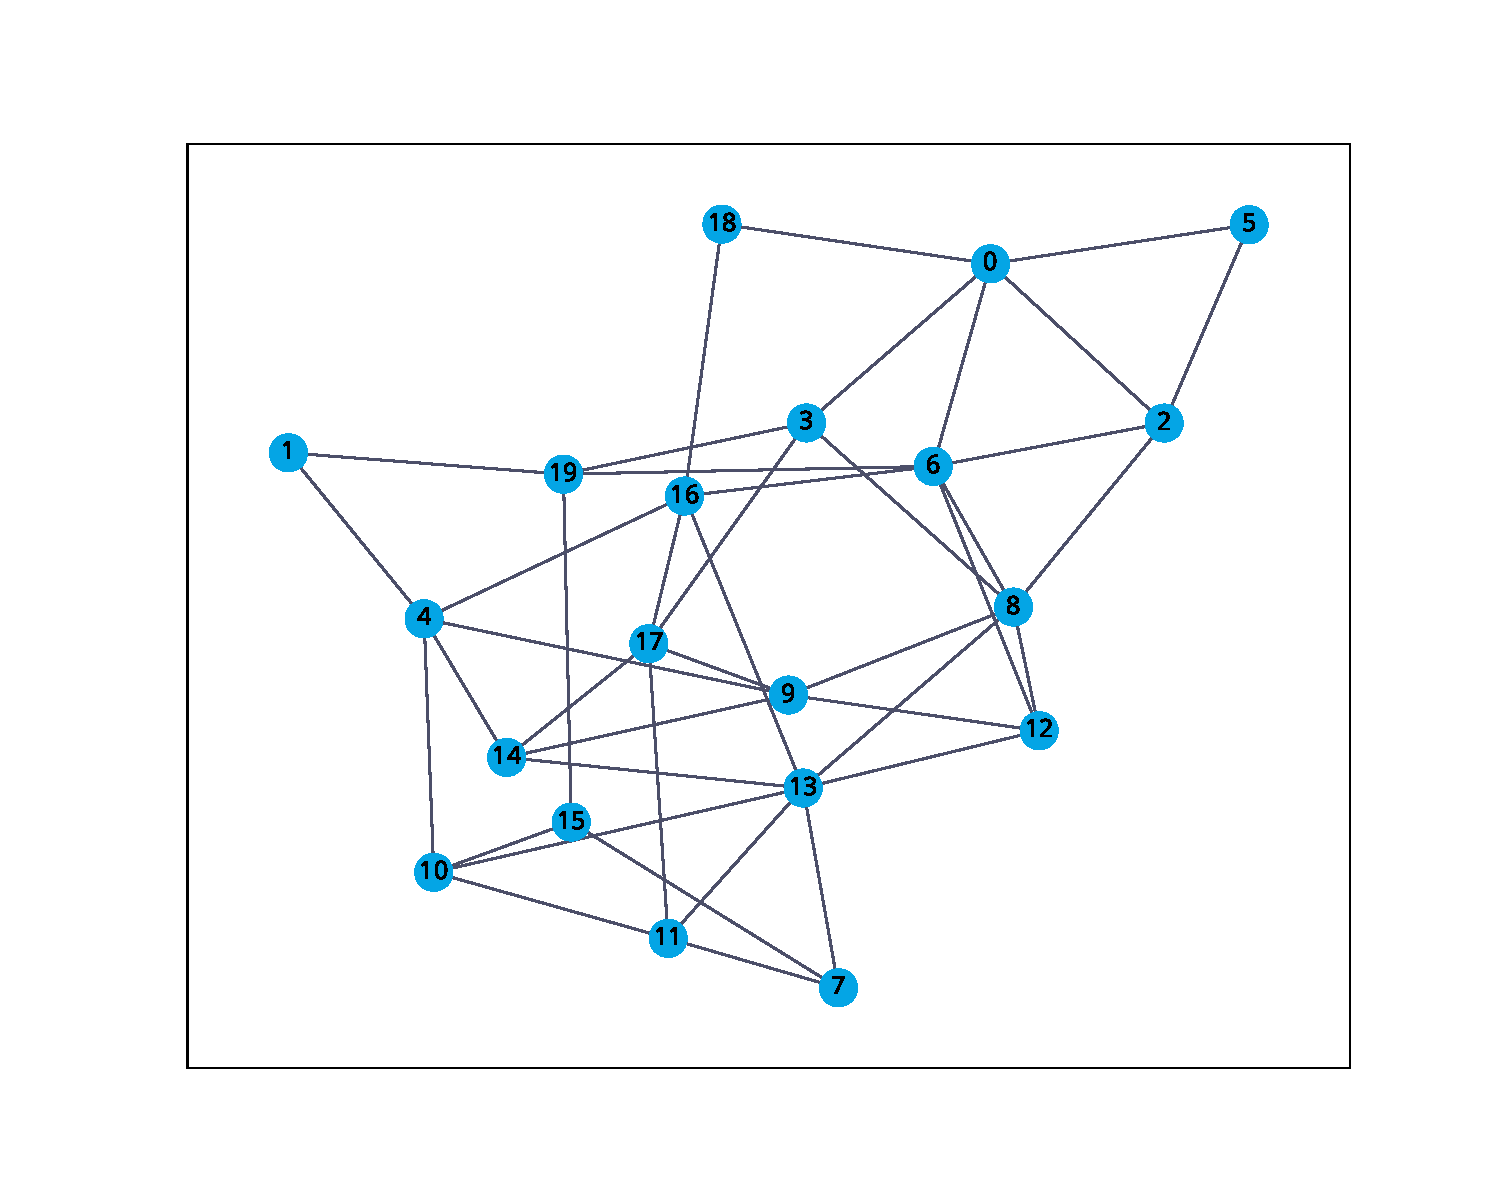
\includegraphics[width=\textwidth]{pictures/plots/20.pdf}
	\caption{\scriptsize$\abs{V} = 20$ nodes and $\abs{E} = 42$ links. (Large)}
	\end{subfigure}
	\label{fig:toynetworks}
\end{figure}
%
% \begin{figure}[!htbp]
% 	\centering
% 	\begin{subfigure}{0.49\textwidth}
% 	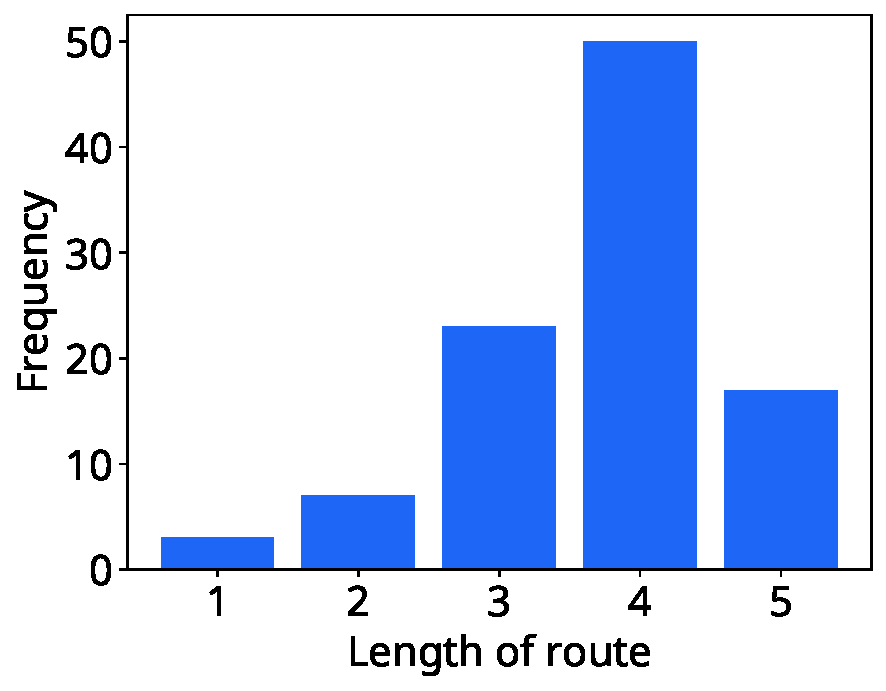
\includegraphics[width=\textwidth]{pictures/plots/topology/route_freq_small.pdf}
% 	\caption{Small}
% 	\end{subfigure}
% 	\begin{subfigure}{0.49\textwidth}
% 	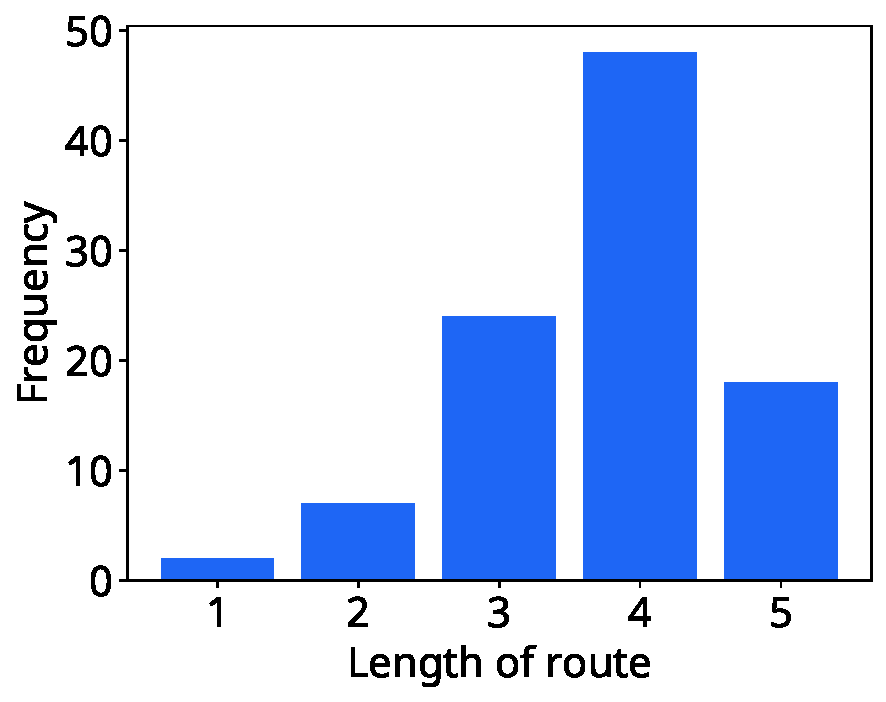
\includegraphics[width=\textwidth]{pictures/plots/topology/route_freq_large.pdf}
% 	\caption{Large}
% 	\end{subfigure}
% 	\caption{The frequency of the length of route (number of links) in each network topology}
% 	\label{fig:toynetworksroutefreq}
% \end{figure}

\end{frame}


\begin{frame}{Numerical Results: Performance}
\begin{itemize}
    \item Blocking ratio:
    \begin{itemize}
        \item At circuit depth $=1$: 20.7\% vs. 6\% ($k$-SPFF)
        \item At circuit depth $=4$: reduced to 18.0\%
    \end{itemize}
    \item Wavelength usage:
    \begin{itemize}
        \item QAOA (depth 1): 82.4\% vs. 86.9\% ($k$-SPFF)
        \item At depth 4: 79.6\%
    \end{itemize}
    % \item Runtime: QAOA simulation $\gg$ SPFF (exponential scaling)
    % \item Underperformance linked to barren plateau phenomenon \cite{grant2019-barren-plateu, McClean2018-barren-plateu, Cunningham2025-vqc-vqe-barren-plateu-taxonomy-literature-review}
\end{itemize}
\begin{figure}[H]
	\centering
	\begin{subfigure}{0.32\textwidth}
	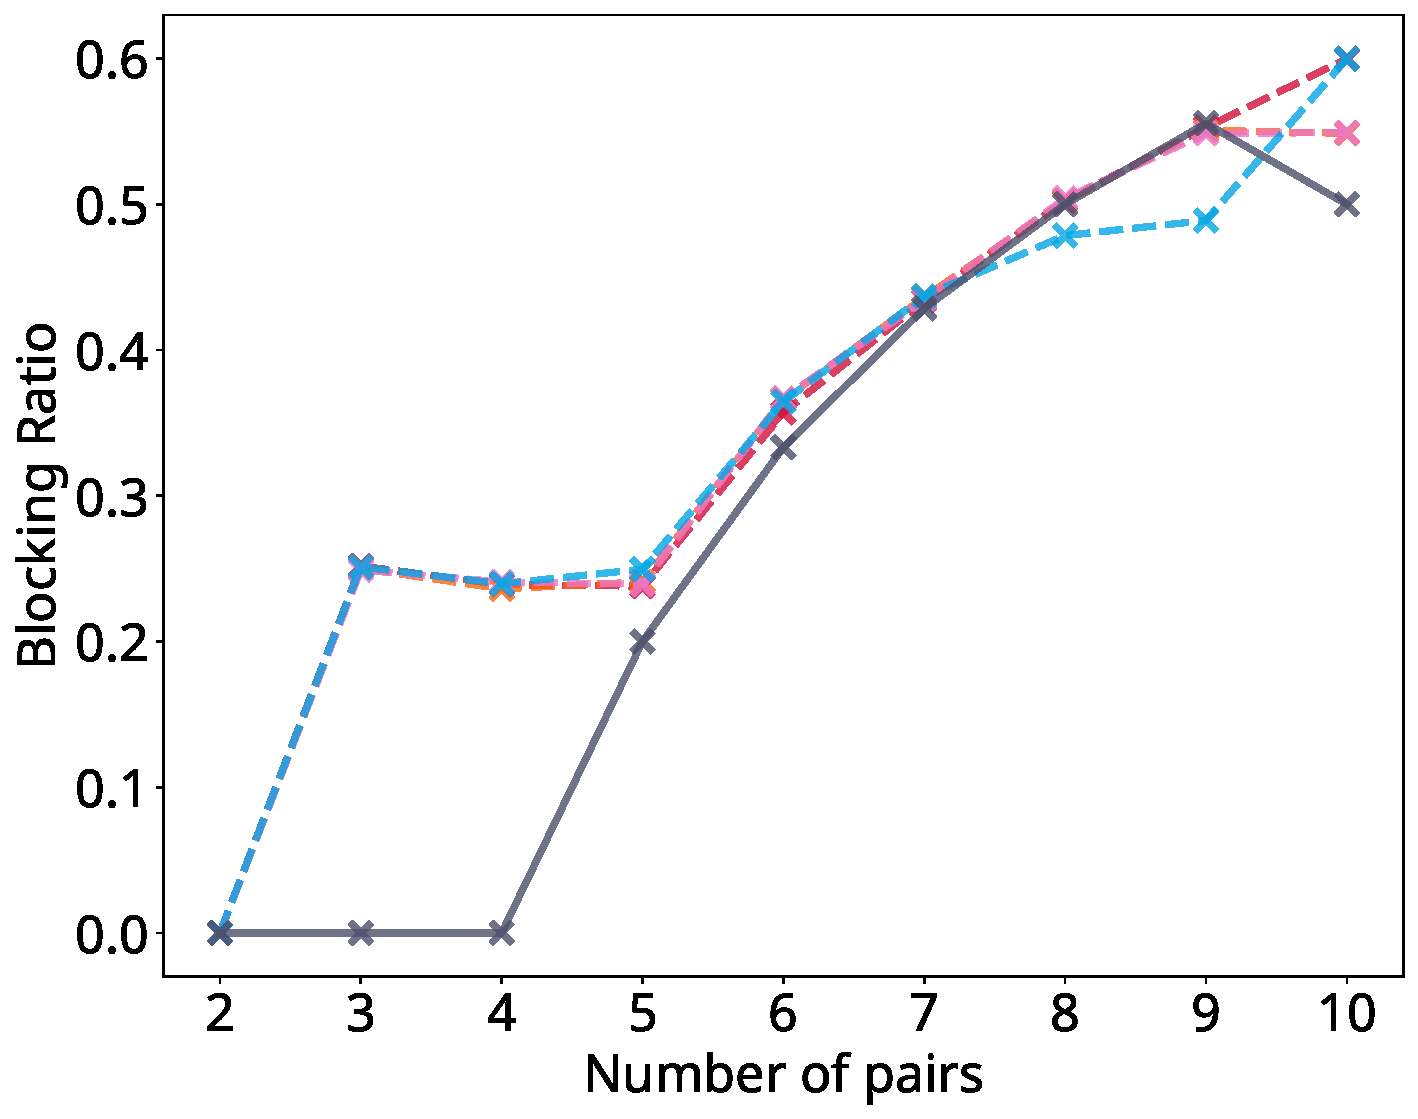
\includegraphics[width=\textwidth]{pictures/plots/n_pairs/x-2-1-s.pdf}
	\caption{$N=2, {\Lambda} = 1$, small topology}
	\end{subfigure}
	\begin{subfigure}{0.32\textwidth}
	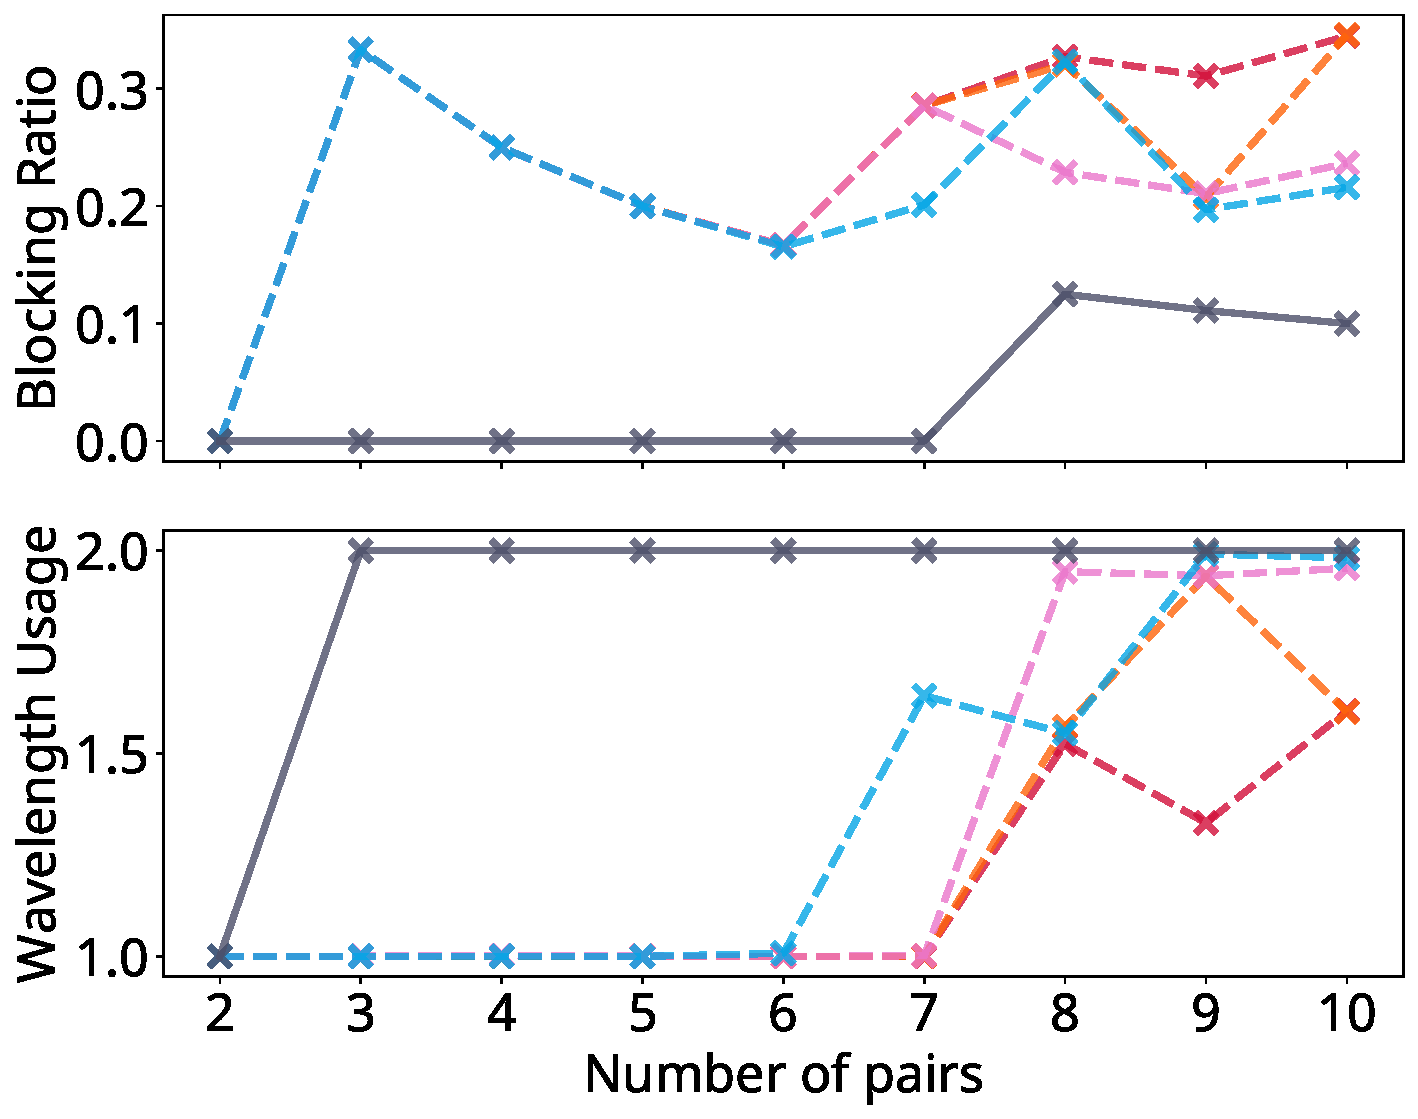
\includegraphics[width=\textwidth]{pictures/plots/n_pairs/x-1-2-m.pdf}
	\caption{$N=1, {\Lambda} = 3$, large topology}
	\label{pairb}
	\end{subfigure}
	\begin{subfigure}{0.32\textwidth}
	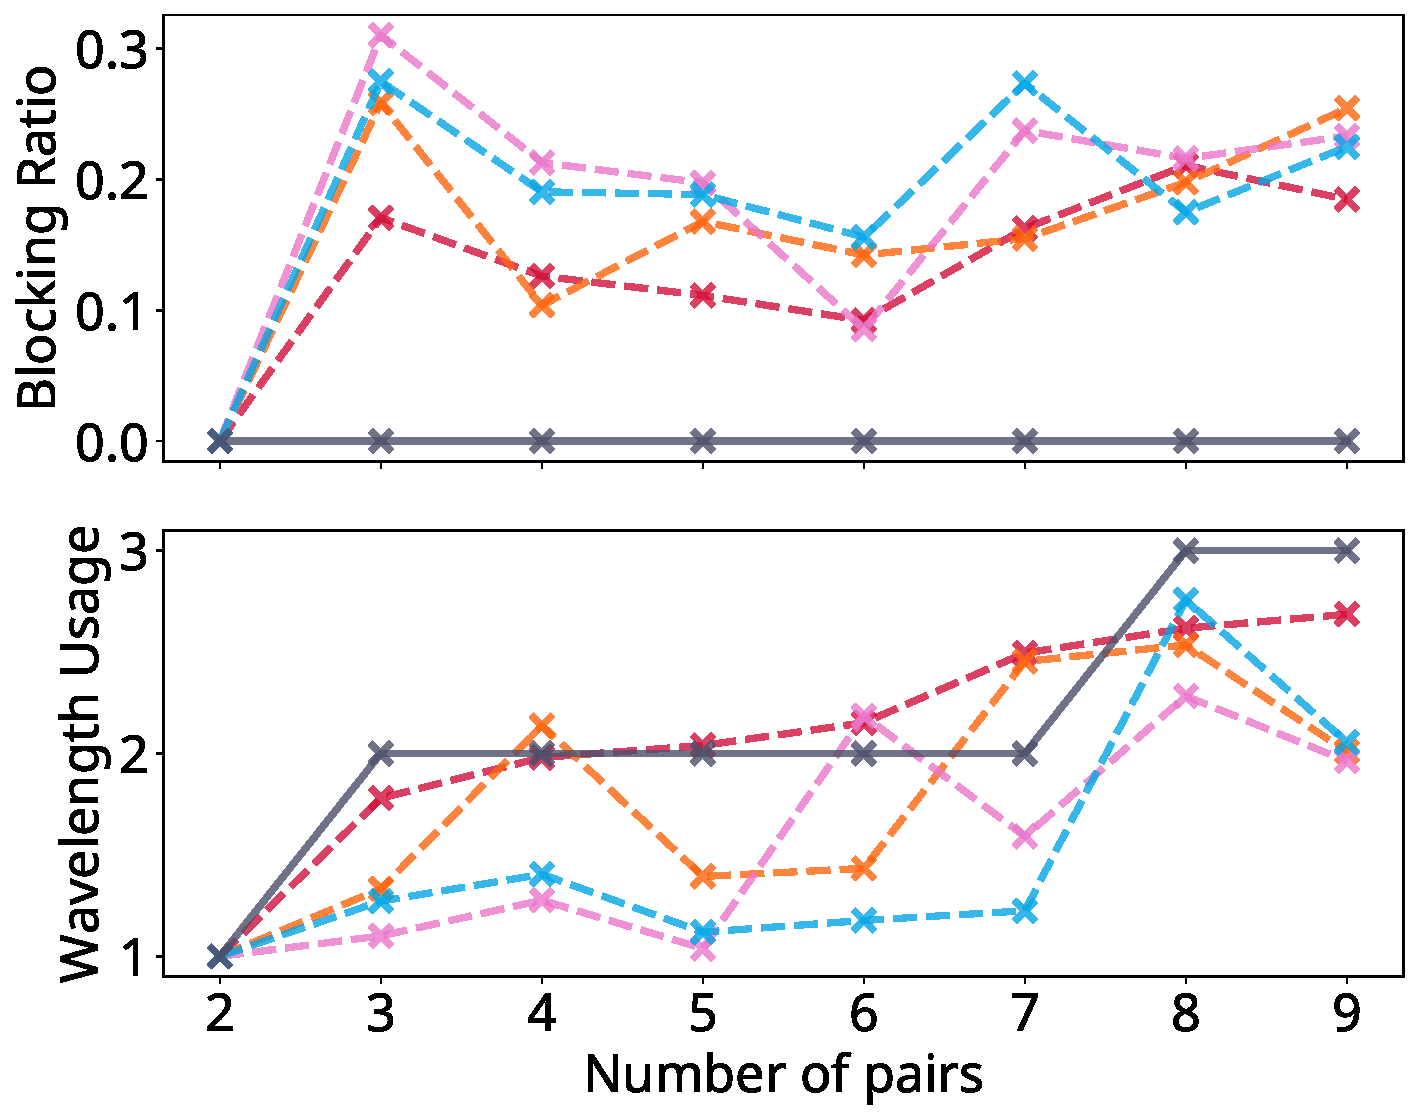
\includegraphics[width=\textwidth]{pictures/plots/n_pairs/x-1-3-m.pdf}
	\caption{$N=1, {\Lambda} = 3$, large topology}
	\label{pairc}
	\end{subfigure}
\caption{\scriptsize The blocking ratio and number of wavelength used.
\protect\reddashed is circuit depth $1$,
\protect\peachdashed is $2$,
\protect\pinkdashed is $3$,
\protect\skydashed is $4$, and
\protect\blackline is k-SPFF.
\label{fig:pairs}
}
\end{figure}

% \includegraphics[width=0.9\textwidth]{pictures/plotfigs/runtime.pdf}
\end{frame}


\begin{frame}{Numerical Results}{Effect of the modified cost function}
% \begin{itemize}
    % \item Original cost function: $ f(\mathbf{x}) = f_{\text{collision}} + f_{\text{wavelength}} $
    % \item Observation: wavelength penalty biases towards fewer wavelengths, ↑ blocking
    \textbf{Modification:} set $f_{\text{wavelength}} =0$. \\
    \textbf{Blocking ratio:} $\downarrow$ by $\sim$3.25\%, \textbf{Wavelength usage:} $\uparrow$ by $\sim$17\%\\
    \textbf{Top rows:} before cost function modification, \textbf{bottom row:} after
    % \item QAOA still underperforms baseline but trade-off becomes clearer
% \end{itemize}
    \begin{figure}[H]
\centering
\begin{subfigure}{0.32\textwidth}
	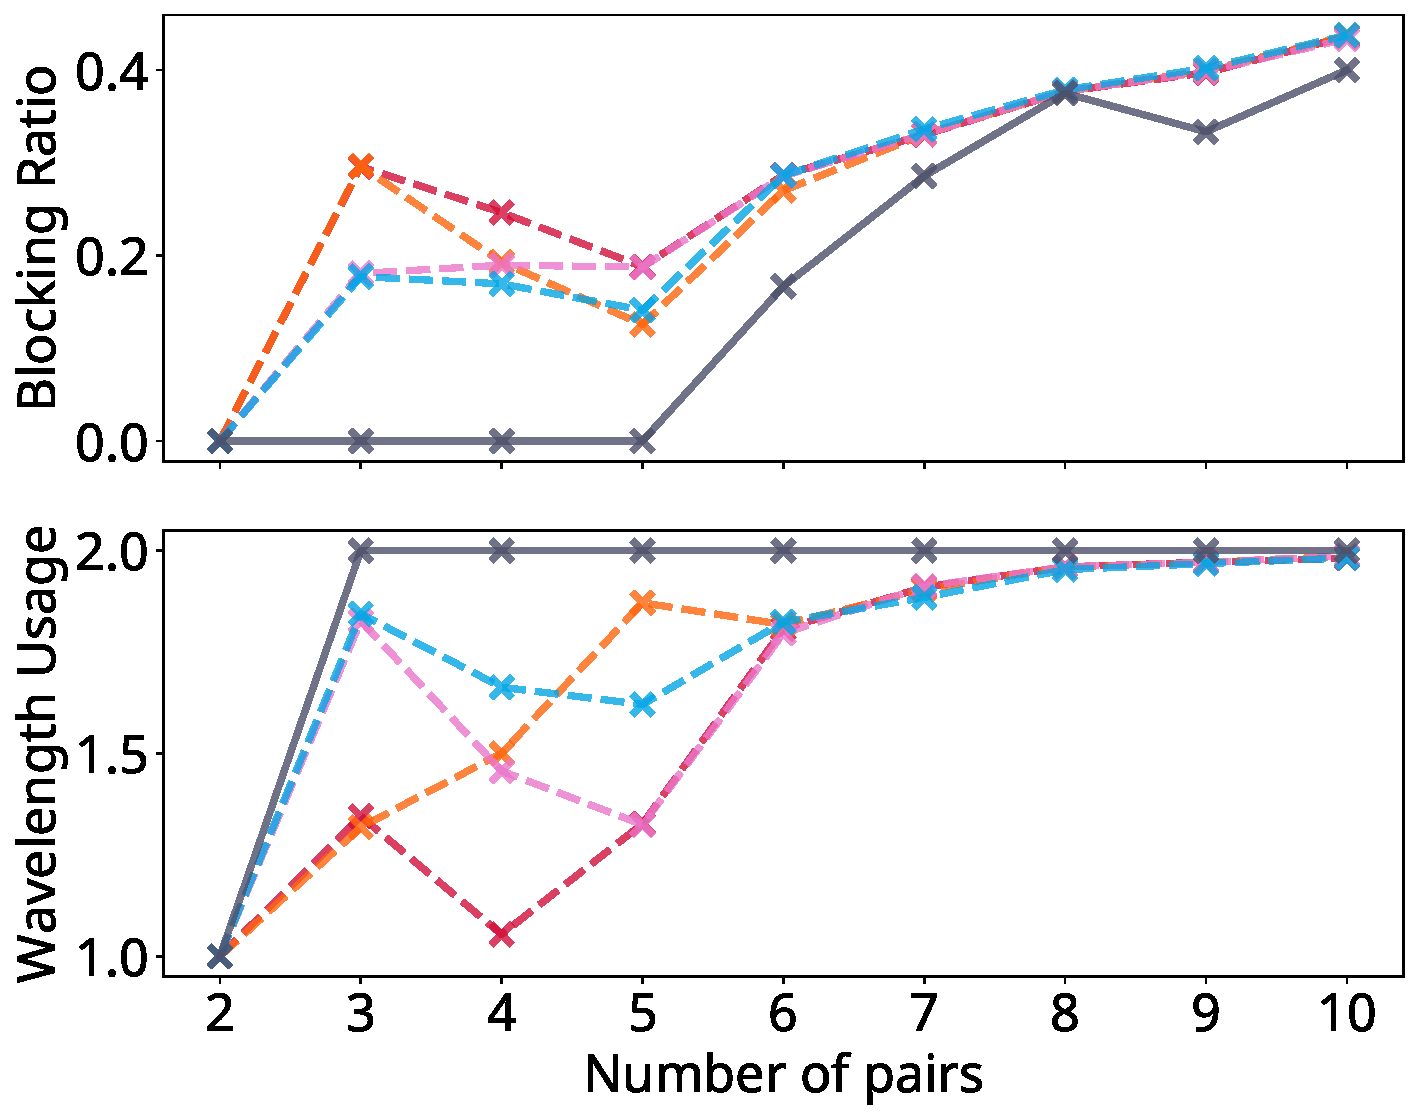
\includegraphics[width=\textwidth]{pictures/plots/n_pairs/x-1-2-s.pdf}
	% \caption{$N=1, \abs{\Lambda} = 2$, small topology}
\end{subfigure}
\begin{subfigure}{0.32\textwidth}
	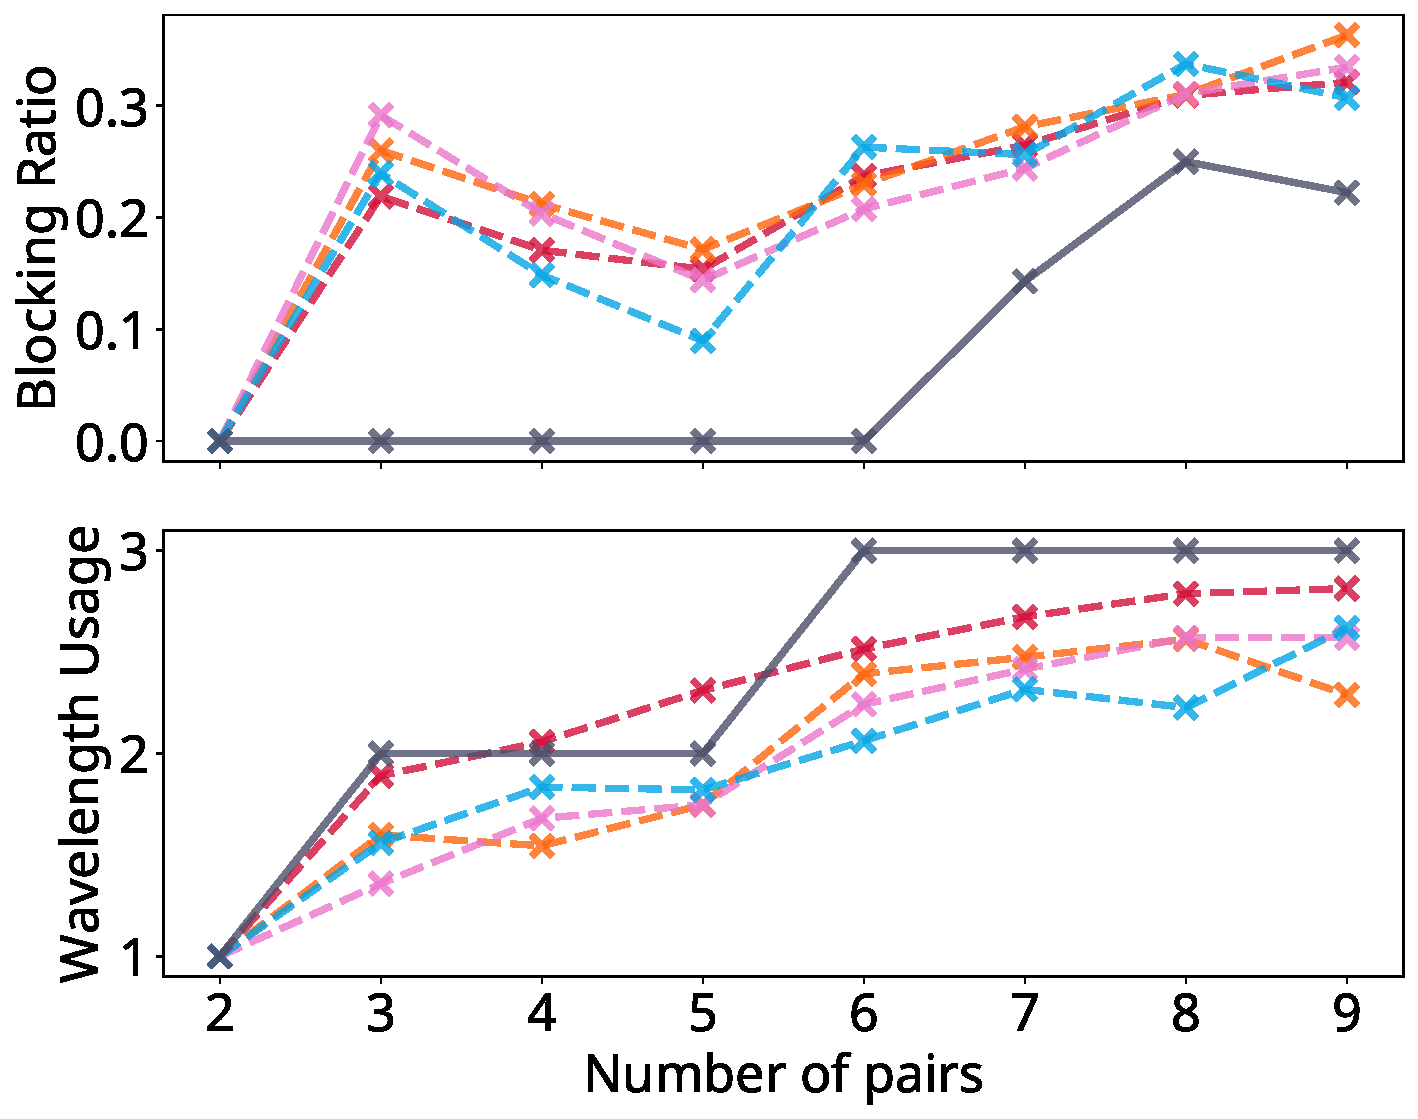
\includegraphics[width=\textwidth]{pictures/plots/n_pairs/x-1-3-s.pdf}
	% \caption{$N=1, \abs{\Lambda} = 3$, small topology}
\end{subfigure}
\begin{subfigure}{0.32\textwidth}
	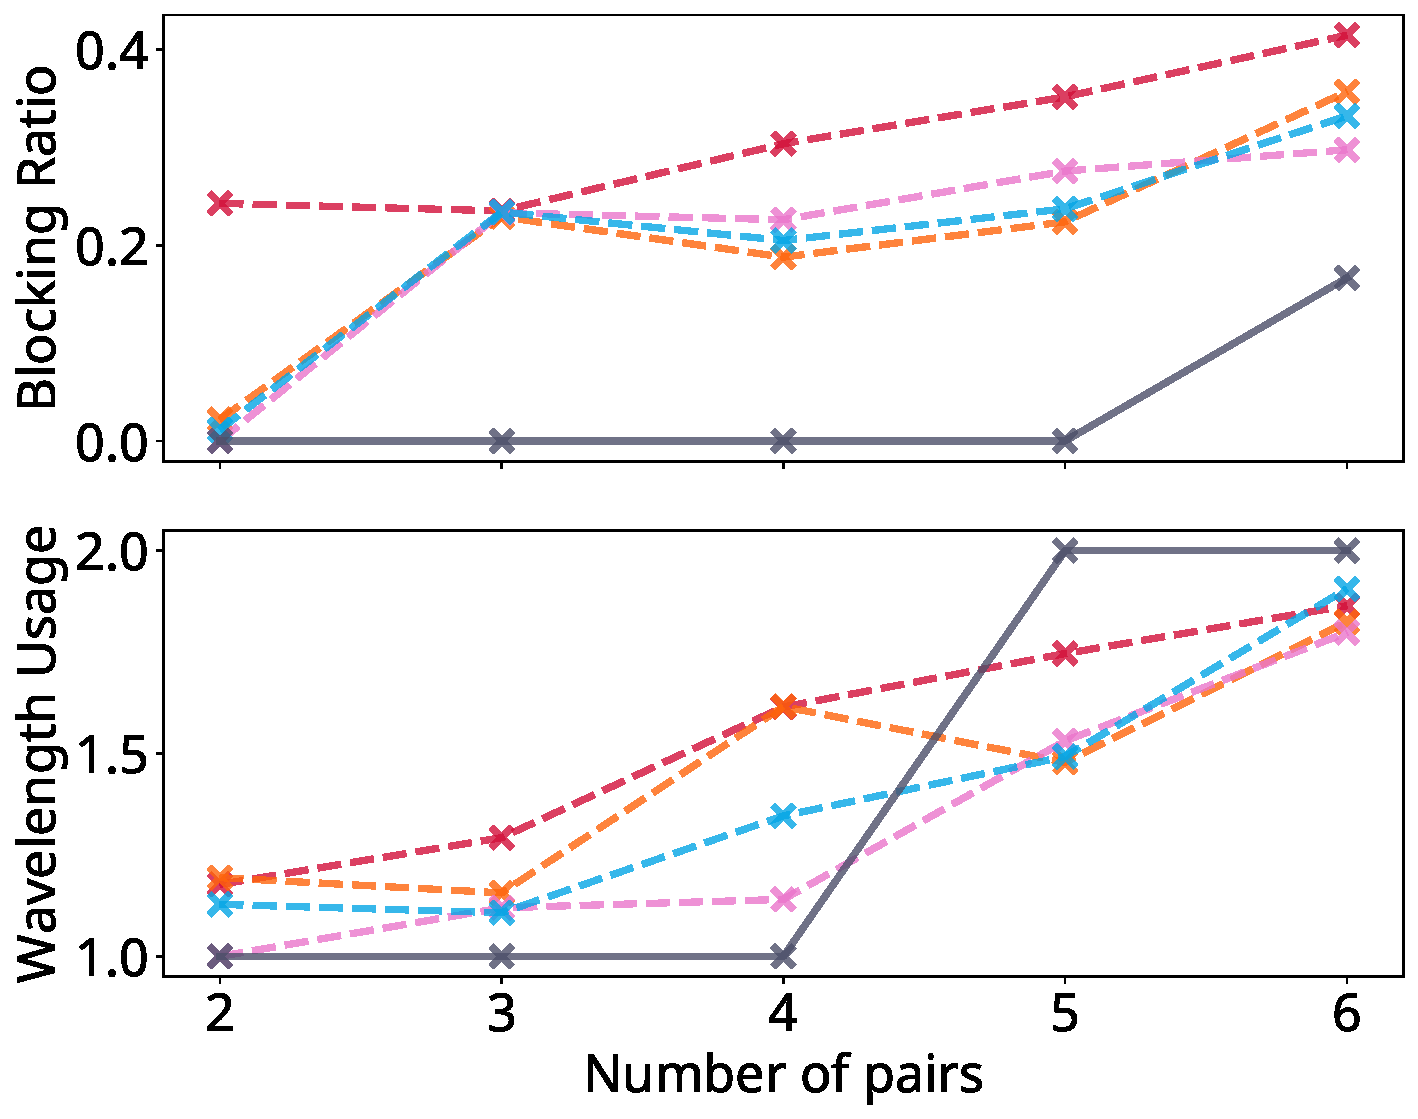
\includegraphics[width=\textwidth]{pictures/plots/n_pairs/x-2-2-s.pdf}
	% \caption{$N=2, \abs{\Lambda} = 2$, small topology}
\end{subfigure}
% \caption{Before}
	\label{fig:pairs_before}
\end{figure}

\begin{figure}[H]
	\centering
\begin{subfigure}{0.32\textwidth}
	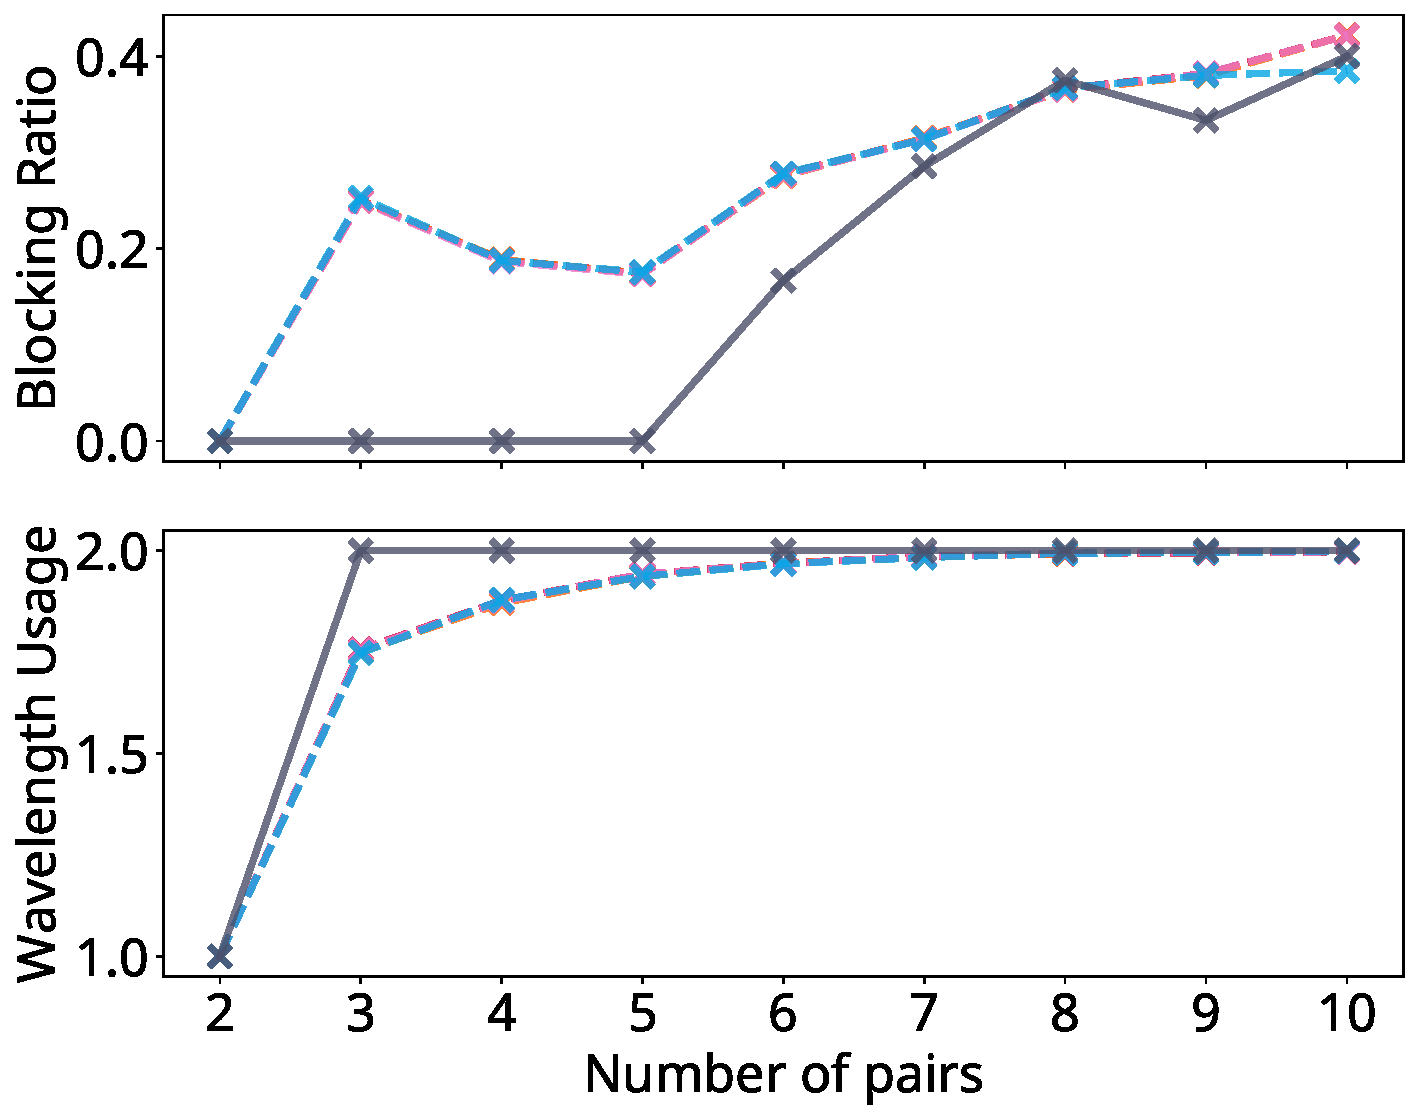
\includegraphics[width=\textwidth]{pictures/plots/n_pairs/cc/x-1-2-s.pdf}
	\caption{\scriptsize $N=1, \abs{\Lambda} = 2$, small topology}
\end{subfigure}
\begin{subfigure}{0.32\textwidth}
	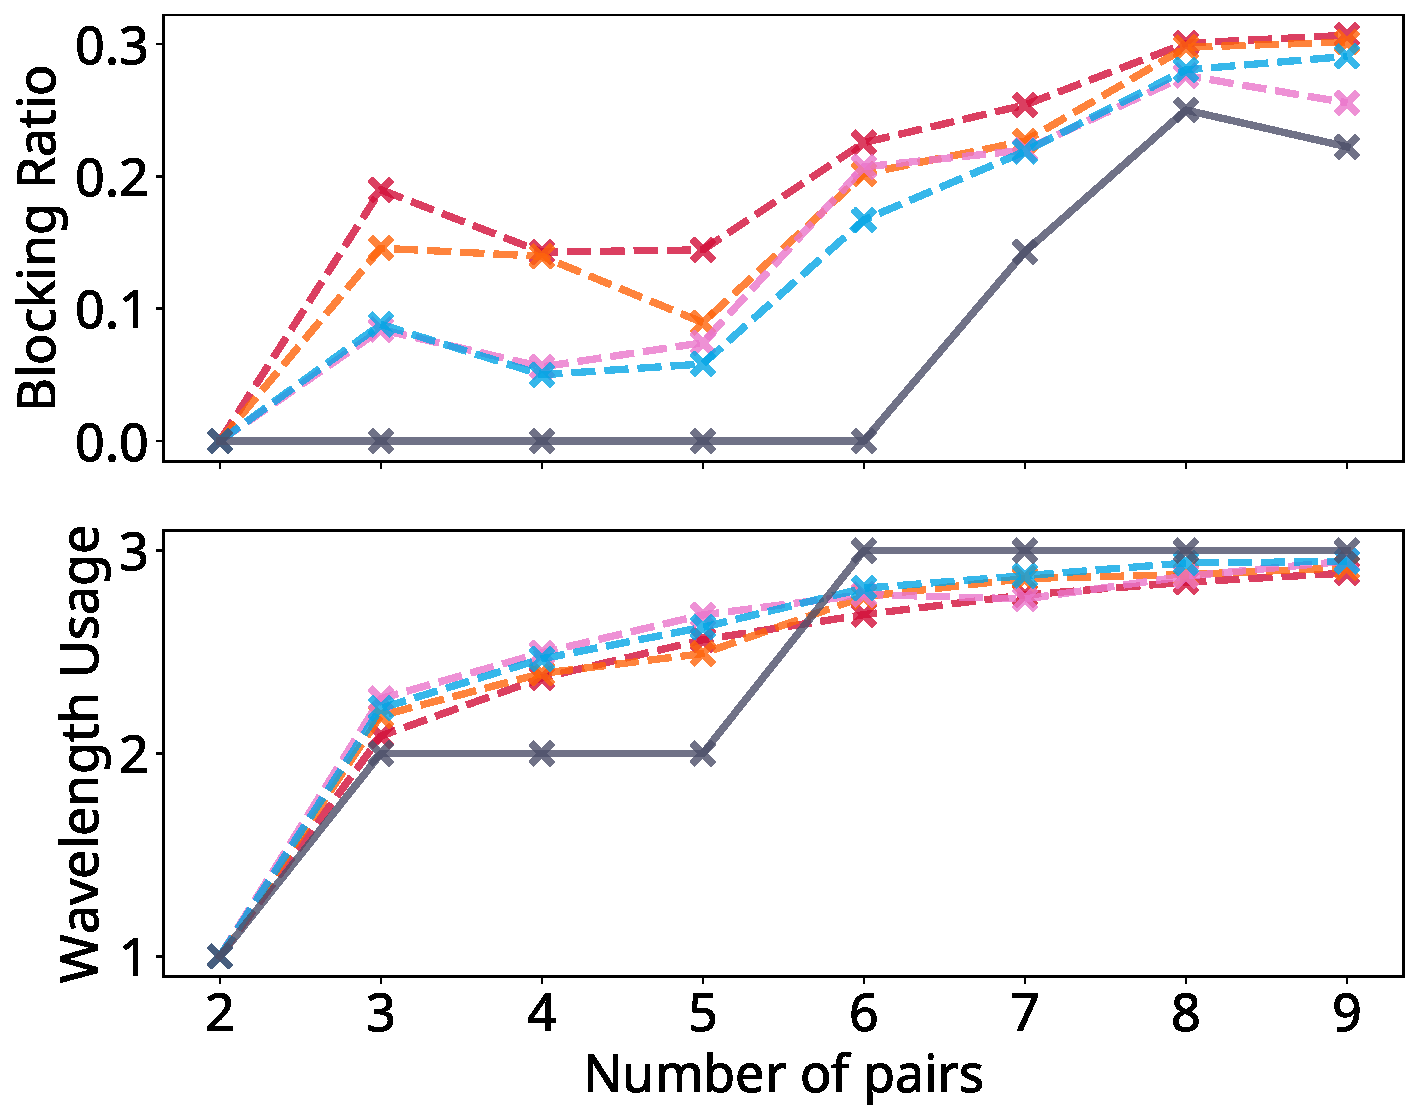
\includegraphics[width=\textwidth]{pictures/plots/n_pairs/cc/x-1-3-s.pdf}
	\caption{\scriptsize $N=1, \abs{\Lambda} = 3$, small topology}
\end{subfigure}
\begin{subfigure}{0.32\textwidth}
	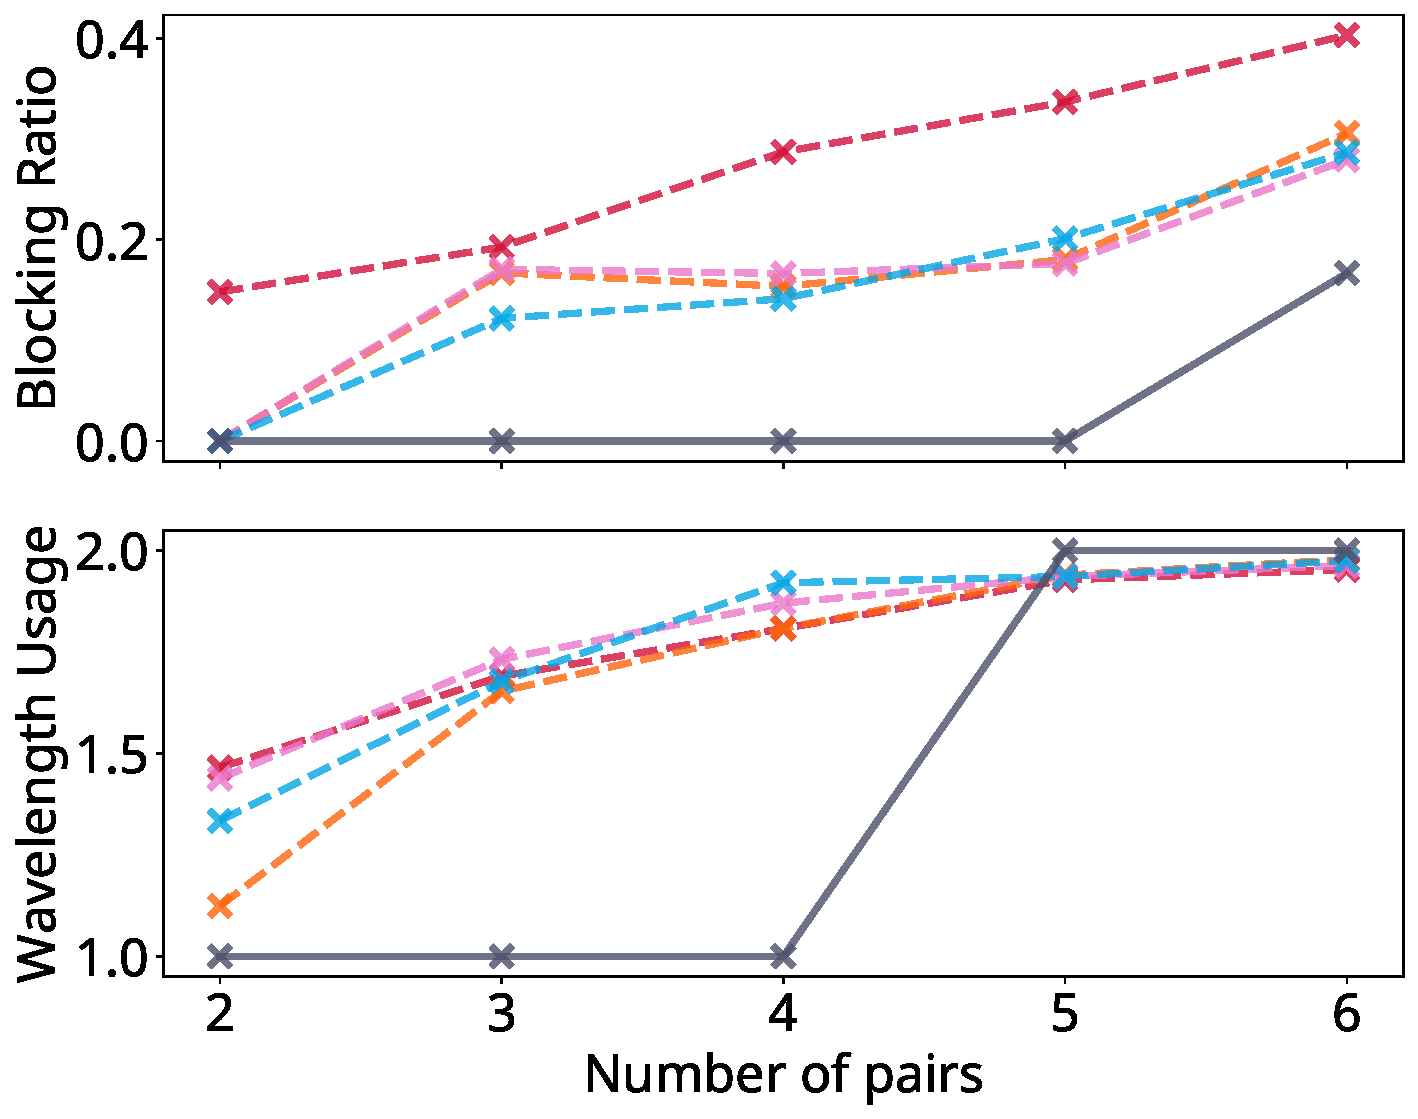
\includegraphics[width=\textwidth]{pictures/plots/n_pairs/cc/x-2-2-s.pdf}
	\caption{\scriptsize$N=2, \abs{\Lambda} = 2$, small topology}
\end{subfigure}
% \caption{The blocking probability and number of wavelength used.
% \protect\reddashed represents $p=1$
% \protect\peachdashed represents $p=2$
% \protect\pinkdashed represents $p=3$
% \protect\skydashed represents $p=4$
% \protect\blackline represents SPFF
% }
% \caption{\scriptsize After}
\label{fig:cc_pairs}
\end{figure}

\end{frame}

\begin{frame}{Quality of Solutions: Distribution Analysis}
\begin{itemize}
    % \item QAOA produces a \textbf{distribution} over feasible states.
    \item Many sampled solutions are low-quality $\Rightarrow$ expected performance pulled down.
    \item Occasionally samples high-quality solutions (better than heuristic).
    % \item Probability of obtaining a “good” solution decreases with problem size.
    \item For small instances ($<20$ qubits), $\sim$10 measurement shots are sufficient to reach $>95\%$ confidence of finding a better solution.
\end{itemize}
\begin{figure}[H]
\centering
\begin{minipage}{.48\textwidth}
  \centering
	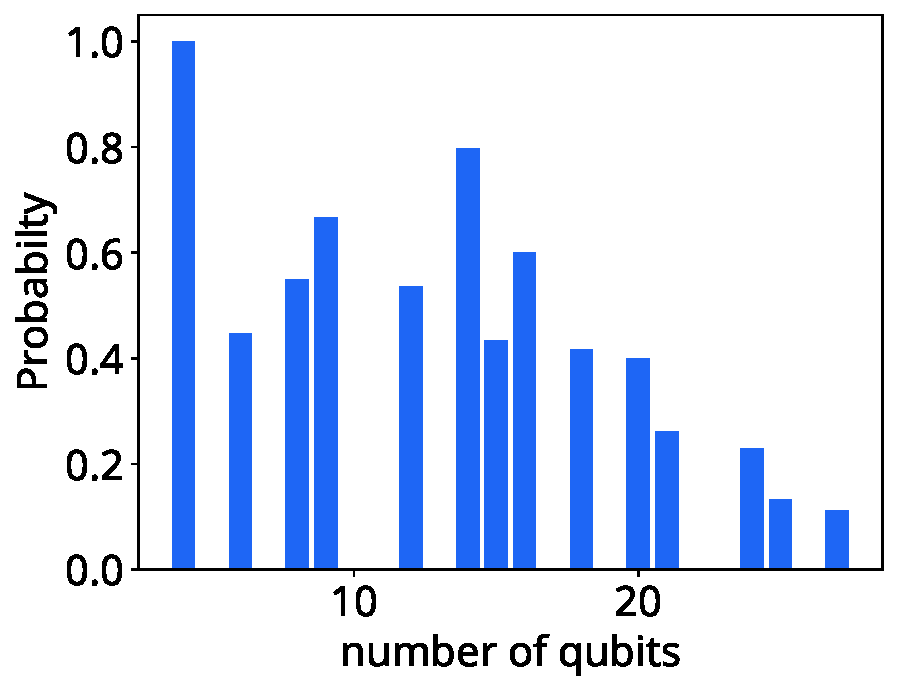
\includegraphics[width=\textwidth]{pictures/plots/prob/prob.pdf}
  % \captionof{figure}{The probability that the measured state will have lower blocking ratio when compared to the k-SPFF algorithm.}
	\label{fig:probprob}
\end{minipage}%
\hfill
\begin{minipage}{.48\textwidth}
  \centering
  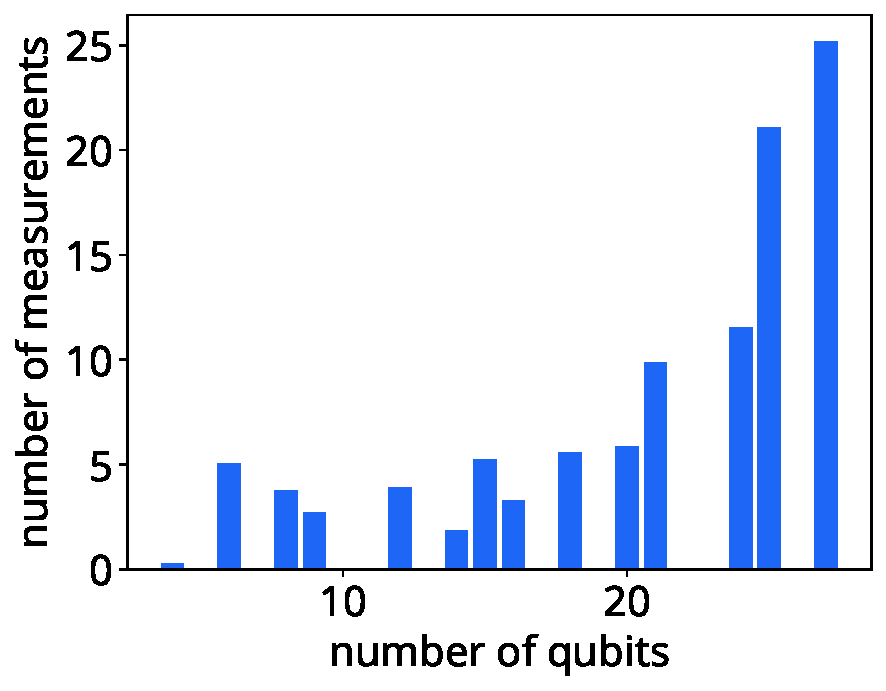
\includegraphics[width=\textwidth]{pictures/plots/prob/num.pdf}
  % \captionof{figure}{The number of measurements required to measure a state with lower blocking ratio when compared to the k-SPFF algorithm 95\% of the time.}
	\label{fig:probnum}
\end{minipage}
\end{figure}


\end{frame}


\begin{frame}{Numerical Results: Two-steps scheme}
\begin{itemize}
        \item Joint formulation $\Rightarrow$ up to 20\% lower blocking
        \item Also uses fewer wavelengths than two-step scheme
        \item Confirms benefit of joint optimisation
\end{itemize}
\begin{figure}[!htbp]
\centering
\begin{subfigure}{0.49\textwidth}
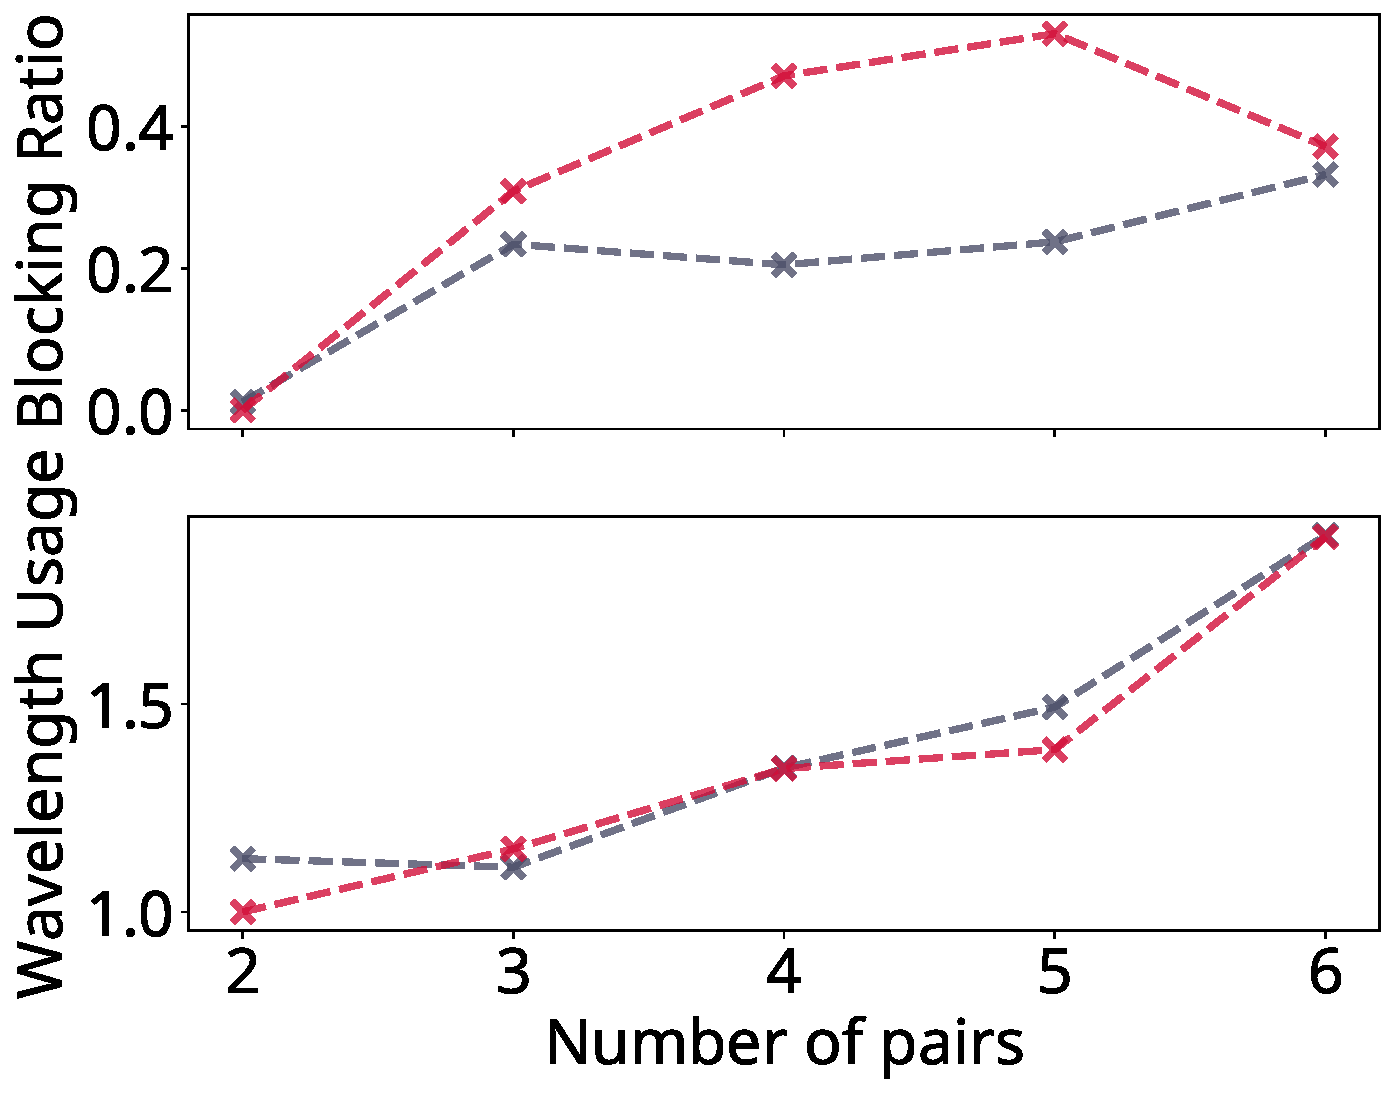
\includegraphics[width=\textwidth]{pictures/plots/rawa/n_pairs/x-2-2-s.pdf}
	\caption{$\abs{P}=2, \abs{\Lambda} = 2$, small topology}
\end{subfigure}
\begin{subfigure}{0.49\textwidth}
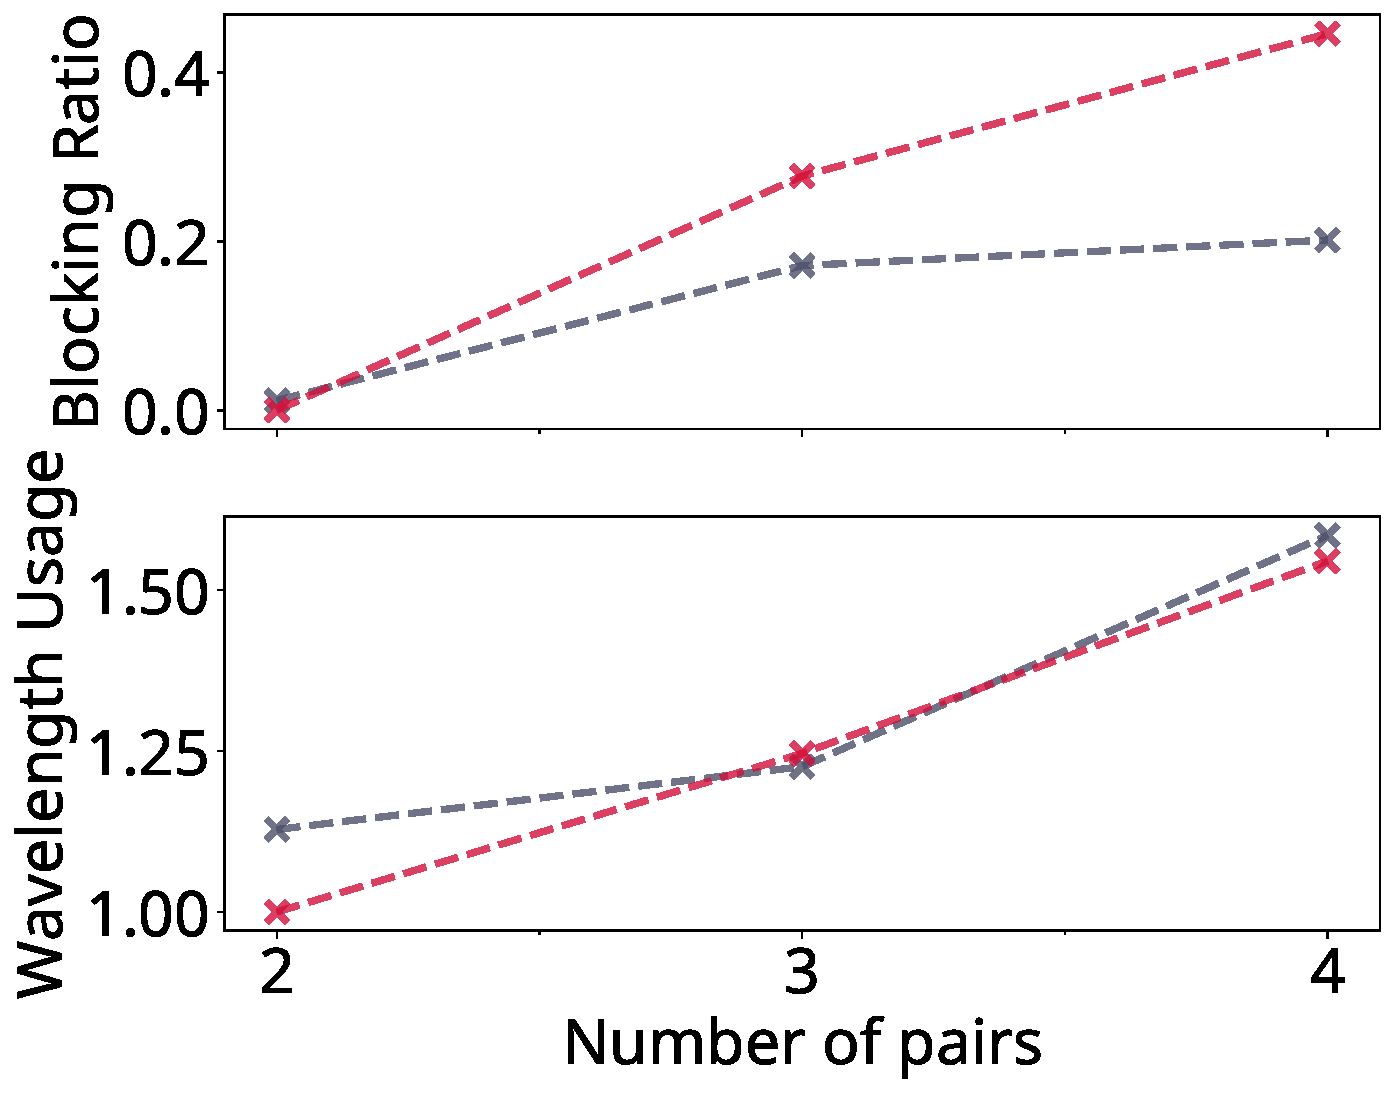
\includegraphics[width=\textwidth]{pictures/plots/rawa/n_pairs/x-2-3-s.pdf}
	\caption{$\abs{P}=2, \abs{\Lambda} = 3$, small topology}
\end{subfigure}
\caption{%The blocking probability and number of wavelength used.
\protect\reddashed is the joint RWA formulation, and 
\protect\blackdashed is the two-steps formulation.
}
\label{fig:rawa}
\end{figure}

\end{frame}
